% Use only LaTeX2e, calling the article.cls class and 12-point type.

\documentclass[12pt]{article}

% Users of the {thebibliography} environment or BibTeX should use the
% scicite.sty package, downloadable from *Science* at
% www.sciencemag.org/about/authors/prep/TeX_help/ .
% This package should properly format in-text
% reference calls and reference-list numbers.
%%%%%
\usepackage{latexsym,amssymb}
\usepackage{amsmath}
\usepackage{graphicx,times}
%\usepackage{psfig}
\usepackage{psfrag}
\usepackage{subfigure}
\usepackage{epstopdf}
\usepackage{CJK}
\usepackage{booktabs}
%%%%%%
\usepackage{scicite}

% Use times if you have the font installed; otherwise, comment out the
% following line.

\usepackage{times}

% The preamble here sets up a lot of new/revised commands and
% environments.  It's annoying, but please do *not* try to strip these
% out into a separate .sty file (which could lead to the loss of some
% information when we convert the file to other formats).  Instead, keep
% them in the preamble of your main LaTeX source file.


% The following parameters seem to provide a reasonable page setup.

\topmargin 0.0cm
\oddsidemargin 0.2cm
\textwidth 16cm
\textheight 21cm
\footskip 1.0cm


%The next command sets up an environment for the abstract to your paper.

\newenvironment{sciabstract}{%
\begin{quote} \bf}
{\end{quote}}


% If your reference list includes text notes as well as references,
% include the following line; otherwise, comment it out.

\renewcommand\refname{References and Notes}

% The following lines set up an environment for the last note in the
% reference list, which commonly includes acknowledgments of funding,
% help, etc.  It's intended for users of BibTeX or the {thebibliography}
% environment.  Users who are hand-coding their references at the end
% using a list environment such as {enumerate} can simply add another
% item at the end, and it will be numbered automatically.

\newcounter{lastnote}
\newenvironment{scilastnote}{%
\setcounter{lastnote}{\value{enumiv}}%
\addtocounter{lastnote}{+1}%
\begin{list}%
{\arabic{lastnote}.}
{\setlength{\leftmargin}{.22in}}
{\setlength{\labelsep}{.5em}}}
{\end{list}}


% Include your paper's title here

\title{Causality Analysis from grey haze to lung cancer}


% Place the author information here.  Please hand-code the contact
% information and notecalls; do *not* use \footnote commands.  Let the
% author contact information appear immediately below the author names
% as shown.  We would also prefer that you don't change the type-size
% settings shown here.

\author
{Sanqing Hu,$^{1\ast}$ Xiaoxue Liu,$^{1}$ Jianhai Zhang,$^{1}$ Wanzeng Kong,$^{1}$\\
\\
\normalsize{$^{1}$College of Computer Science, Hangzhou Dianzi University,}\\
\normalsize{Hangzhou, 310018, China}\\
\normalsize{$^\ast$To whom correspondence should be addressed; E-mail:  sqhu@hdu.edu.cn.}
}

% Include the date command, but leave its argument blank.

\date{}



%%%%%%%%%%%%%%%%% END OF PREAMBLE %%%%%%%%%%%%%%%%



\begin{document}

% Double-space the manuscript.

\baselineskip24pt

% Make the title.

\maketitle



% Place your abstract within the special {sciabstract} environment.

\begin{sciabstract}
In recent years, with the rapid development of economy, China and other countries in the world suffer from serious environmental pollution, such as haze pollution. At the same time, lung cancer is one of the highest incidence of malignant tumors, and its incidence rate also shows a rising trend. The main component in haze includes the atmospheric aerosol particles. When one breathes, aerosol may hinder pulmonary gas exchange, can even penetrate the lungs and cause serious harm to human health. Dui Wu et al. ({\it 1\/})has shown that the mortality of lung cancer is correlated to the concentration of aerosol particles in Guangzhou city, China. However, it does not reflect that the heavy concentration of the aerosol particles can cause lung cancer. In this paper we apply our recently proposed new causality method ({\it 2\/}) and confirm that grey haze has important causal influence on the increasing mortality of lung cancer. Also we confirm that grey haze at low concentration leads to lung cancer with longer lag time, grey haze at high concentration leads to lung cancer with shorter lag time. The widely used Granger causality method ({\it 3\/}) ({\it 4\/}) cannot derive such a conclusion. In the face of increasingly serious worsening haze environment in large area, our finding will undoubtedly make decision maker realize the necessity and urgency to take all measures to control haze environment. All human economic and social activities should be based on people's health, fear of life as the premise, otherwise we will soon pay a heavy price for blood.
\end{sciabstract}


% In setting up this template for *Science* papers, we've used both
% the \section* command and the \paragraph* command for topical
% divisions.  Which you use will of course depend on the type of paper
% you're writing.  Review Articles tend to have displayed headings, for
% which \section* is more appropriate; Research Articles, when they have
% formal topical divisions at all, tend to signal them with bold text
% that runs into the paragraph, for which \paragraph* is the right
% choice.  Either way, use the asterisk (*) modifier, as shown, to
% suppress numbering.

\section*{Introduction}

In recent years, the incidence and mortality of lung cancer worldwide have shown an obviously rising trend. According to the latest data released by China Cancer Center, the incidence and mortality of lung cancer rank first among all cancers and meanwhile the growing trend continues. What worries us most is that the incidence of lung cancer takes place in younger people. So far there is no definitive conclusion about the cause of lung cancer, among which genetic variation is the internal cause and basis of cancer, and we still have no effective method to intervene the internal cause. It is a common idea that smoking is the most important cause of lung cancer, studies suggest that 80\% of the lung cancer results from smoking (some studies suggest 90\%). But since the smoking rate in China shows a  relatively stable tendency in past 30 years, the incidence rate of lung cancer has still continued to soar. This fact makes us consider other factors, particularly, the impact of persistently deteriorated air pollution on the lung cancer in recent years.

Numbers of studies have indicated high risk for lung cancer in association with the different level of exposure to
ambient air pollution. For example, in a cohort study of up to 0.5 million people in the 1982-1998 years the American Cancer Society found that fine particulate matter (PM2.5) increases by an average annual concentration of 10 mu g/m3, the population of lung cancer mortality will rise by $8\%$ (RR=1.08,95\%CI=1.01-1.16) ({\it 5\/}). David E. Abbey et al. showed that residence and work location in areas of high ambient air pollution with long periods are associated with increased mortality ({\it 6\/}). Christopher H et al. found that exposure to PM10, PM2.5, and ozone ambient may increase the risk for pulmonary exacerbations and increase the rate of change in lung function in the CF population ({\it 7\/}). The very large multicentre study shows an association between exposure to particulate matter air pollution and the incidence of lung cancer ({\it 8\/}). Fine PM with an aerodynamic diameter �� 2.5��m (PM2.5) was associated with lung cancer mortality in  cohort studies from the United States ({\it 9\/}). The study made by Ole Raaschou-Nielsen et al. indicates associations between risk for lung cancer and different markers of air pollution from traffic near the residence which is in line with the weight of the epidemiologic evidence to date({\it 10\/}).J.Mumford et al. analysed the lung cancer and indoor air pollution in Xuan Wei,China and suggested an etiologic link between domestic smoky coal burning and lung cancer in Xuan Wei where the lung cancer mortality is among China's highest({\it 11\/}).Lester B. Lave and Eugene P. Seskin show a close association between air pollution and ill health. The evidence is extremely good for some diseases (such as bronchitis and lung cancer)({\it 12\/}). According to a research last for years made by Guangzhou institute of tropical marine meteorological's researcher shows under the condition of stable tendency of smoking rate for years,the frequently occurrence of haze weather has correlation with the rapid increasing trend of lung cancer incidence in Guangzhou city,China({\it 1\/}).

Among so many kinds of air pollution,the grey haze is one of most severe pollution. The main component in haze includes the atmospheric aerosol particles. When one breathes, aerosol may hinder pulmonary gas exchange, can even penetrate the lungs and cause serious harm to human health.On February 28, 2015,a famous documentary made by former CCTV host Jing Chai which is at her own expense named "under the dome" published on the Internet,immediately raised wide public concern.Till March 2, video has been broadcast more than 200 million times.The video focuses on the danger of grey haze and gives a vivid classes for the people suffering from gray haze pollution.The grey haze weather has biggest impact on the respiratory system as it contacts with the environment most frequently.At the same time,the haze weather abates the ultraviolet ray and enhances the activity of bacteria in the air.Fine particulate matter will "bring" bacteria and viruses to the depths of the respiratory system and cause infection.As the component of the grey haze,aerosol particles can scatter and absorb the solar radiation.Most of the atmospheric aerosol can be absorbed in the human respiratory tract,especially the submicron particle will deposition in the lower or upper respiratory tract and alveoli and then result in lung cancer.Although the individual internal mechanism of lung cancer is not clear so far,what is for sure is that these pests and carcinogens deposite slowly in the body, when accumulated to a certain degree the body's immune system began to fall and eventually lead to lung cancer.

Granger causality is one of most well-known method to reveal causal relationship.Due to its simplicity and easy understanding,it has been widely applied to the economy ({\it 13\/}),neural science({\it 14\/})({\it 15\/}),genetics({\it 16\/}) and climate studies({\it 17\/})({\it 18\/}). Sanqing Hu indicates the limitations of Granger causality and then derive the conception of new causality({\it 2\/}).Granger causality in the time domain can't correctly reveal impact strength from a time sequence to another time series,at the same time the Granger causality in frequency domain has internal defects due to the use of transfer function(inverse matrix).Both Granger causality and new causality use the method of proportion,but they are defined on the two different equations,Granger causality is a part of the new causality and new causality is a natural extension of Granger causality.Sanqing Hu has confirmed the new causality is more accurate to reveal true inherit causal relationship than Granger causality with a large number of examples({\it 19\/})({\it 20\/}).


In this passage,we establish the linear regression model of lung cancer mortality and aerosol extinction coefficient(AEC) and then we apply new causality to confirm the grey haze is an important external cause of lung cancer.On average,lung cancer mortality has 8 years lag relationship with AEC which is consistent with the results of Dui Wu et al({\it 1\/}).Meanwhile,we derive AEC at low concentration leads to lung cancer with longer lag time, AEC at high concentration leads to lung cancer with shorter lag time.

\section*{Data analysis methods and results}
\paragraph*{Granger causality and new causality.}
Granger causality can be simply described as follows:consider two time series, $X_1$ and $X_2$,if the adding of the previous value of $X_2$ improves the prediction of the current value of $X_1$,then we say $X_2$ has a causal relationship with $X_1$.The autoregressive model can be presented as follows:
\begin{equation}\left\{
\begin{aligned}
X_{1,t}=\sum\limits_{j=1}^{m}{\bf a}_{1,j}X_{1,t-j}+\varepsilon_{1,t} ,~ var(\varepsilon_{1,t})=\Sigma_1 \\
X_{2,t}=\sum\limits_{j=1}^{m}{\bf a}_{2,j}X_{2,t-j}+\varepsilon_{2,t} ,~ var(\varepsilon_{2,t})=\Gamma_1 \\
\end{aligned}
\right.
\label{z1}
\end{equation}

Of which ,$a_{1,j}$,$a_{2,j}$ indicate the coefficient of the autoregression model, $t = 0,1,\cdots ,N$($N$ is sample size),$m$ represents the order of the model,$\varepsilon_{1,t}$,$\varepsilon_{2,t}$ are the noise terms which are uncorrelated over time,$\Sigma_1$ and $\Gamma_1$ is respectively defined by $\sigma_{\varepsilon_{1,t}}^2$ and $\sigma_{\varepsilon_{2,t}}^2$.At this time,the values of noise terms depend on the past value of $X_1$ and $X_2$ respectively.And their joint representations are described as follows:
\begin{equation}\left\{
\begin{aligned}
X_{1,t}=\sum\limits_{j=1}^{m}a_{11,j}X_{1,t-j}+\sum\limits_{j=1}^{m}a_{12,j}X_{2,t-j}+\eta_{1,t} ,~ var(\eta_{1,t})=\Sigma_2\\
X_{2,t}=\sum\limits_{j=1}^{m}a_{21,j}X_{1,t-j}+\sum\limits_{j=1}^{m}a_{22,j}X_{2,t-j}+\eta_{2,t},~ var(\eta_{2,t})=\Gamma_2\\
\end{aligned}
\right.
\label{z2}
\end{equation}

Where $a_{11,j}$,$a_{12,j}$,$a_{21,j}$,$a_{22,j}$ indicate the coefficient of the joint regression model,$m$ is the order of the model, $t = 0,1,\cdots ,N$($N$ indicates the total number of the samples),$\eta_{1,t}$,$\eta_{2,t}$ are the noise terms and here we define $\Sigma_2$,$\Gamma_2$ as the variance of the noise terms.This time,the value of noise terms depend on the past value of both $X_{1,t}$ and $X_{2,t}$.

Granger causality can be formulized below:

\begin{equation}
F_{X_2\rightarrow X_1}=\ln \frac{\Sigma_1}{\Sigma_2}
\label{a1}
\end{equation}


\begin{equation}
F_{X_1\rightarrow X_2}=\ln \frac{\Gamma_1}{\Gamma_2}
\end{equation}

If $\Sigma_2$$<$$\Sigma_1$,then $F_{X_2\rightarrow X_1}>0$ ,that is to say the adding of $X_2$ improved the accuracy of the prediction of $X_1$ which indicates there is some causal relationship from $X_2$ to $X_1$,if $\Sigma_2$$=$$\Sigma_1$, then $F_{X_2\rightarrow X_1}=0$,so there is no causal influence from $X_2$ to $X_1$.Similarly,we can use this criterion to confirm whether $X_1$ has a causal relationship with $X_2$.

However,Sanqing Hu ({\it 2\/}) indicates the shortcomings/limitations of the granger causality and then derive the conception of new causality.According to the formula(2),
$\sum\limits_{j=1}^{m}a_{11,j}X_{1,t-j}$,$\sum\limits_{j=1}^{m}a_{12,j}X_{2,t-j}$
and $\eta_{1,t}$ each plays a role on the contribution of $X_{1,t}$,so the definition of causality from $X_2$ to $X_1$ can be described as is shown below:
\begin{equation}
n_{X_2\rightarrow X_1}=\frac{\sum\limits_{t=m+1}^{N}{(\sum\limits_{j=1}^{m}a_{12,j}X_{2,t-j})}^2}
{\sum\limits_{h=1}^{2}{\sum\limits_{t=m+1}^{N}{(\sum\limits_{j=1}^{m}a_{1h,j}X_{h,t-j})}^2}+\sum\limits_{t=m+1}^{N}\eta_{1,t}^2}
\label{z12}
\end{equation}
or
\begin{equation}
n_{X_2\rightarrow X_1}=\frac{\sum\limits_{t=m+1}^{N}{(\sum\limits_{j=1}^{m}a_{12,j}X_{2,t-j})}^2}
{\sum\limits_{h=1}^{2}{\sum\limits_{t=m+1}^{N}{(\sum\limits_{j=1}^{m}a_{1h,j}X_{h,t-j})}^2}+N\sigma_{\eta_1}^2}
\label{z10}
\end{equation}

Similarly,the casual relationship from $X_1$ to $X_2$ can be described below:

\begin{equation}
n_{X_1\rightarrow X_2}=\frac{\sum\limits_{t=m+1}^{N}{(\sum\limits_{j=1}^{m}a_{21,j}X_{1,t-j})}^2}
{\sum\limits_{h=1}^{2}{\sum\limits_{t=m+1}^{N}{(\sum\limits_{j=1}^{m}a_{2h,j}X_{h,t-j})}^2}+\sum\limits_{t=m+1}^{N}\eta_{2,t}^2}
\end{equation}
or \begin{equation}
n_{X_1\rightarrow X_2}=\frac{\sum\limits_{t=m+1}^{N}{(\sum\limits_{j=1}^{m}a_{21,j}X_{1,t-j})}^2}
{\sum\limits_{h=1}^{2}{\sum\limits_{t=m+1}^{N}{(\sum\limits_{j=1}^{m}a_{2h,j}X_{h,t-j})}^2}+N\sigma_{\eta_2}^2}
\end{equation}


We can only determine whether there is causal relationship between two time series or not from the definition of granger causality which is as formula $(3)$ and $(4)$ shown.We cannot determine whether differnt parts have different contributions to the value of causality.New causality remedy the limitation of Granger causality,from the formula of the definition of the new causality,we can see it can both confirm whether there have causality or not and we can confirm which part contributes most to the value of causality.
\paragraph*{Experimental data}
  We firstly use the research findings made by Xuexi Tie and Dui Wu et al.({\it 1\/})({\it 21\/}) and then extract the data,pictures are shown below.

\begin{figure}[htbp]
%\psfrag{iEEG}[c][c][2]{${\rm iEEG}$}
\vspace{-2.2cm}
\centering
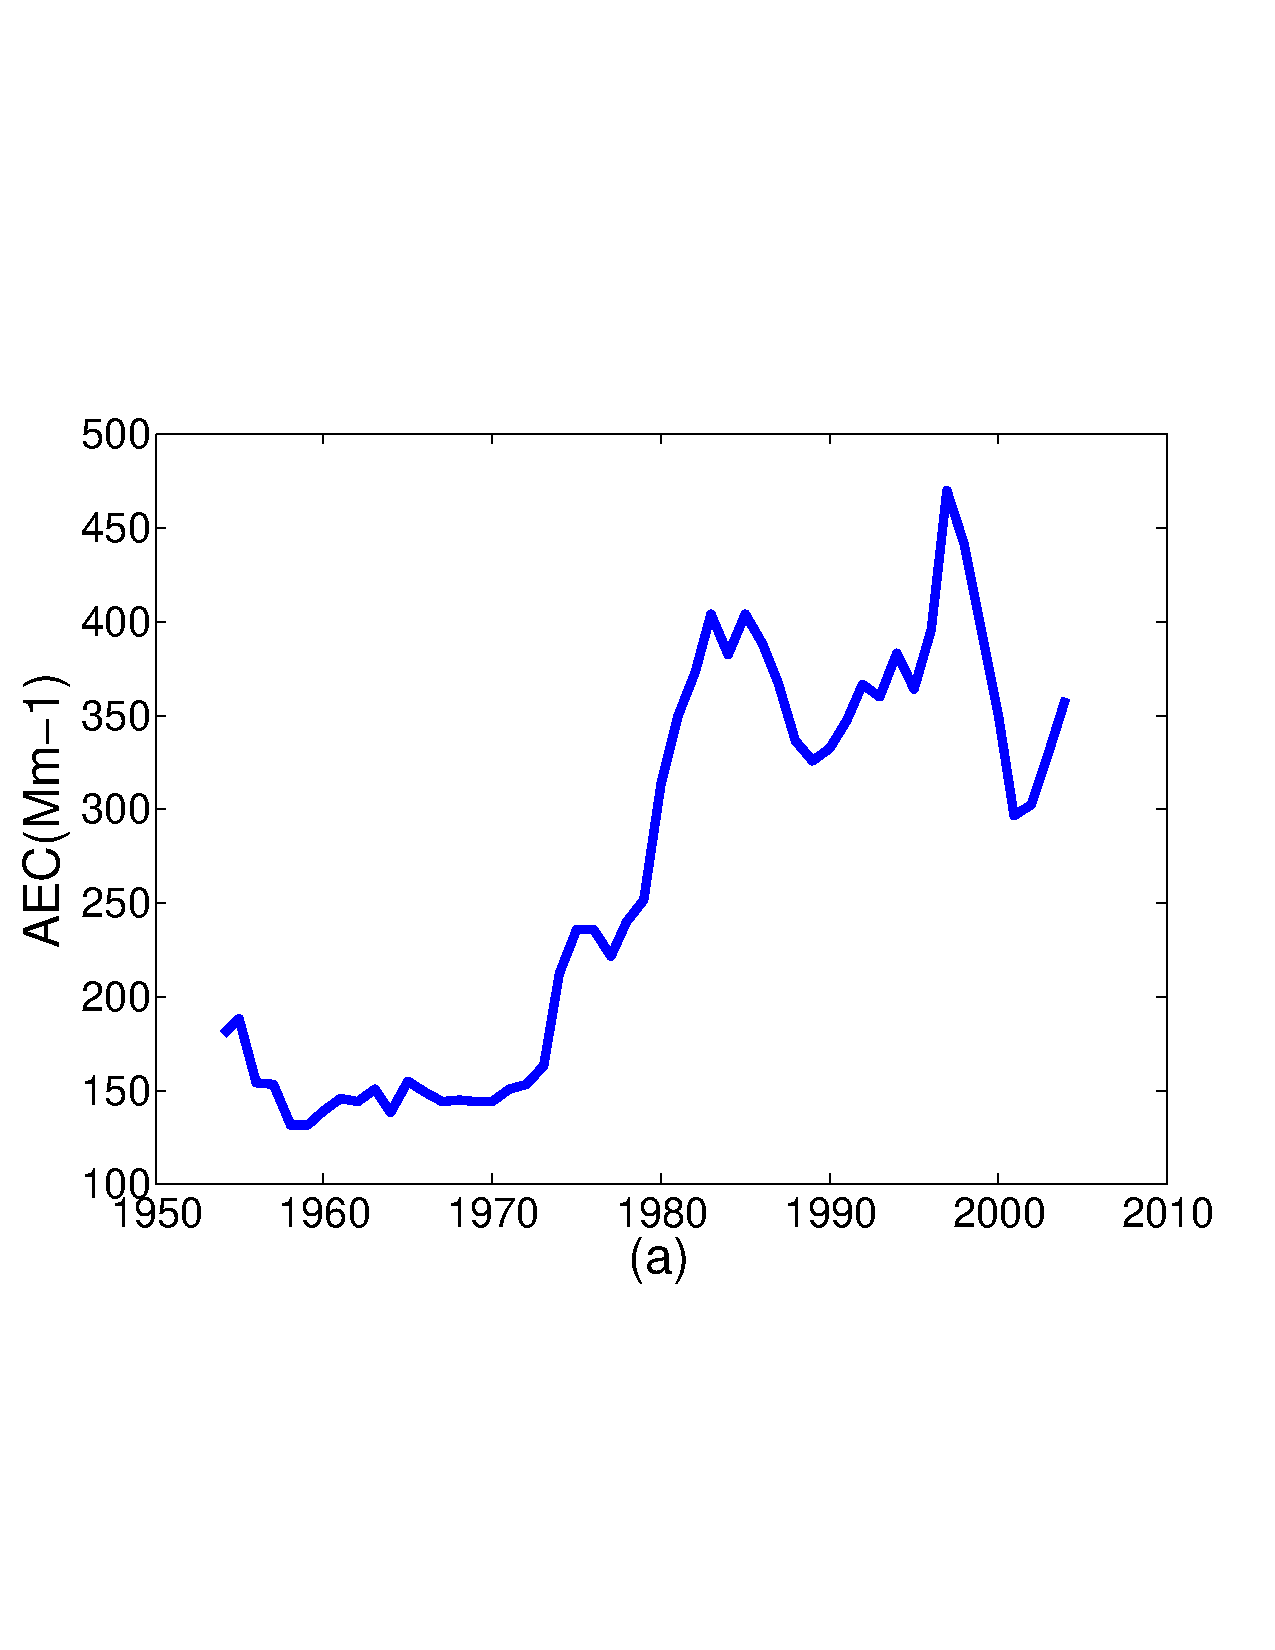
\includegraphics[width=3in]{smog}\hspace{-0.2cm}
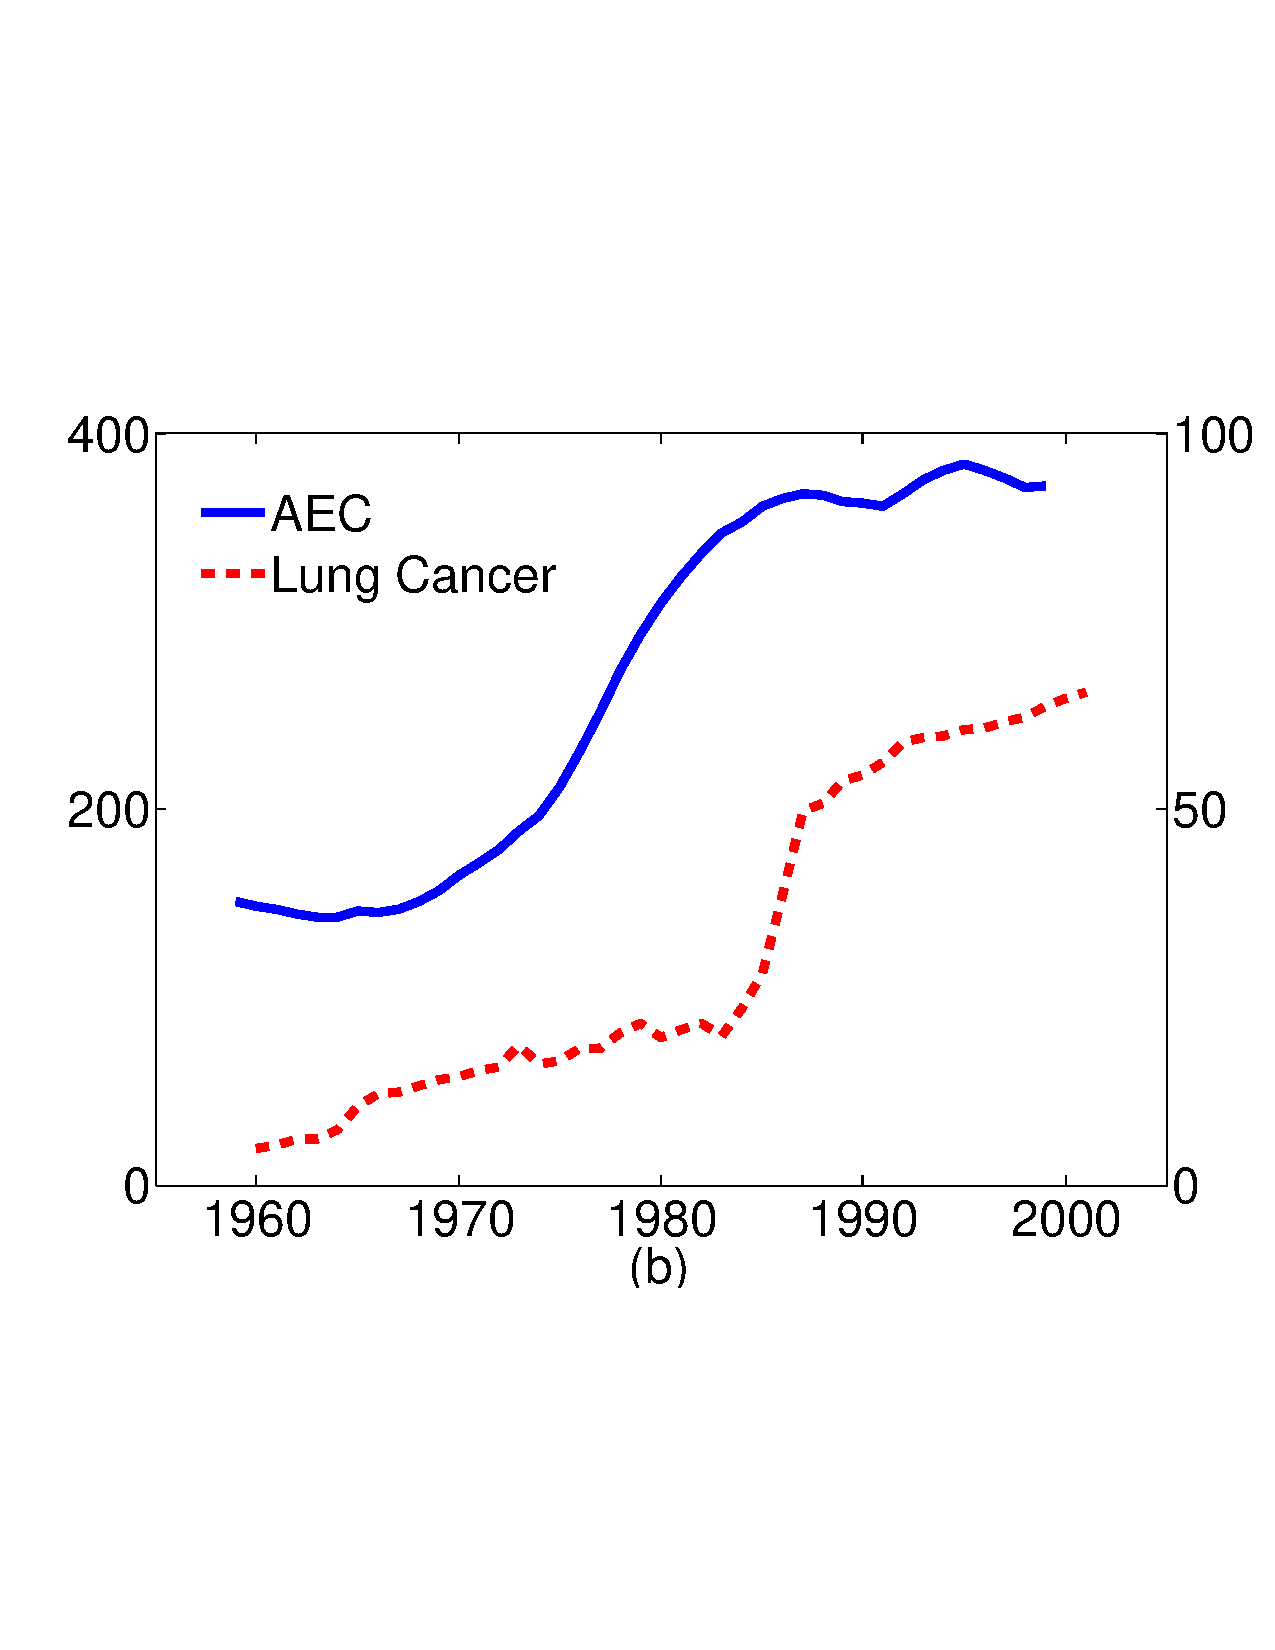
\includegraphics[width=3in]{rawData}
\vspace{-2cm}\\
\caption{(a) raw data of aerosol extinction coefficient(AEC). (b) AEC(10-year moving average) and lung cancer mortality(1/100000).}
\label{f6}
\end{figure}


From (Fig. 1(b)),we can see there is a obvious lag time between lung cancer mortality and aerosol extinction coefficient(As the rapid variations in aerosol level do not have a significant effects on the illness,thus we use a smoothed value of AEC(10-year moving average) as the experimental data).We first get the aerosol extinction coefficient from the year of 1960 to 1999 as the series called $X_2$,then we get the lung cancer mortality relatively which we name $X_1$.Now we want to calculate the causality from AEC to lung cancer,that is to say,to analyse the causality from $X_2$ to $X_1$,on the first step,we calculate the average value of $X_1$,$X_2$,here we define $ \overline X_1$,$ \overline X_2$ as the average value of $X_1$,$X_2$.On the second place,each value of $X_1$ and $X_2$ subtracts the average value of $X_1$,$X_2$ respectively,this way,we get two new time series,$(X_1-\overline X_1)$ and $(X_2-\overline X_2)$,we name the two time series as the new $X_1$ and $X_2$ time series.
\paragraph*{The order selection of linear regression model.}
In the process of constructing a time series regression model, the choice of the order is rather important,it determines the specific functional form of linear regression model.If the order chosen is too big,it will reduce the degrees of freedom and increase the complexity of the calculation.On the contrary,if the chosen order is too small,we will not be able to accurately estimate the model,thus a standard to choose accurate lag order is particularly important(the order represents the value of $m$ in the formula(1)(2)).

  The commonly used regression model order selection criteria is called AIC criterion(Akaike information criterion)({\it22\/})({\it23\/})({\it24\/}).Specific function can be expressed as:
  \begin{equation}
 AIC(m)=Nlog(det(\Sigma))+2mn^2
\end{equation}

 where $N$ indicates the total number of the samples,$m$ represents the lag order of the model,$n$ means the number of variables in the regression model,$\Sigma$ indicates covariance matrix.$AIC(m)$ is the discrete function about order m,the optimal order should make the minimum value of the function value. The max value of m,we use the Schwart(1987) recommended method,the max value of m is defined by $12*(T/100)^{0.25}$($T$ is the total number of samples),here as we use the data from 1960 to 1999,thus the total number is 40,then the maximum of m equals to $12*(40/100)^{0.25}=9.543$
,so the max value of $m$ is 9.Next we calculate the AIC value where $m$ equals to 1 to 9.The results is as (Fig. 2) shown.We can see the the optimal order of the model is 9 as the AIC value  reachs the minimum.

\begin{figure}[htbp]
%\psfrag{iEEG}[c][c][2]{${\rm iEEG}$}
\vspace{-2.2cm}
\centering
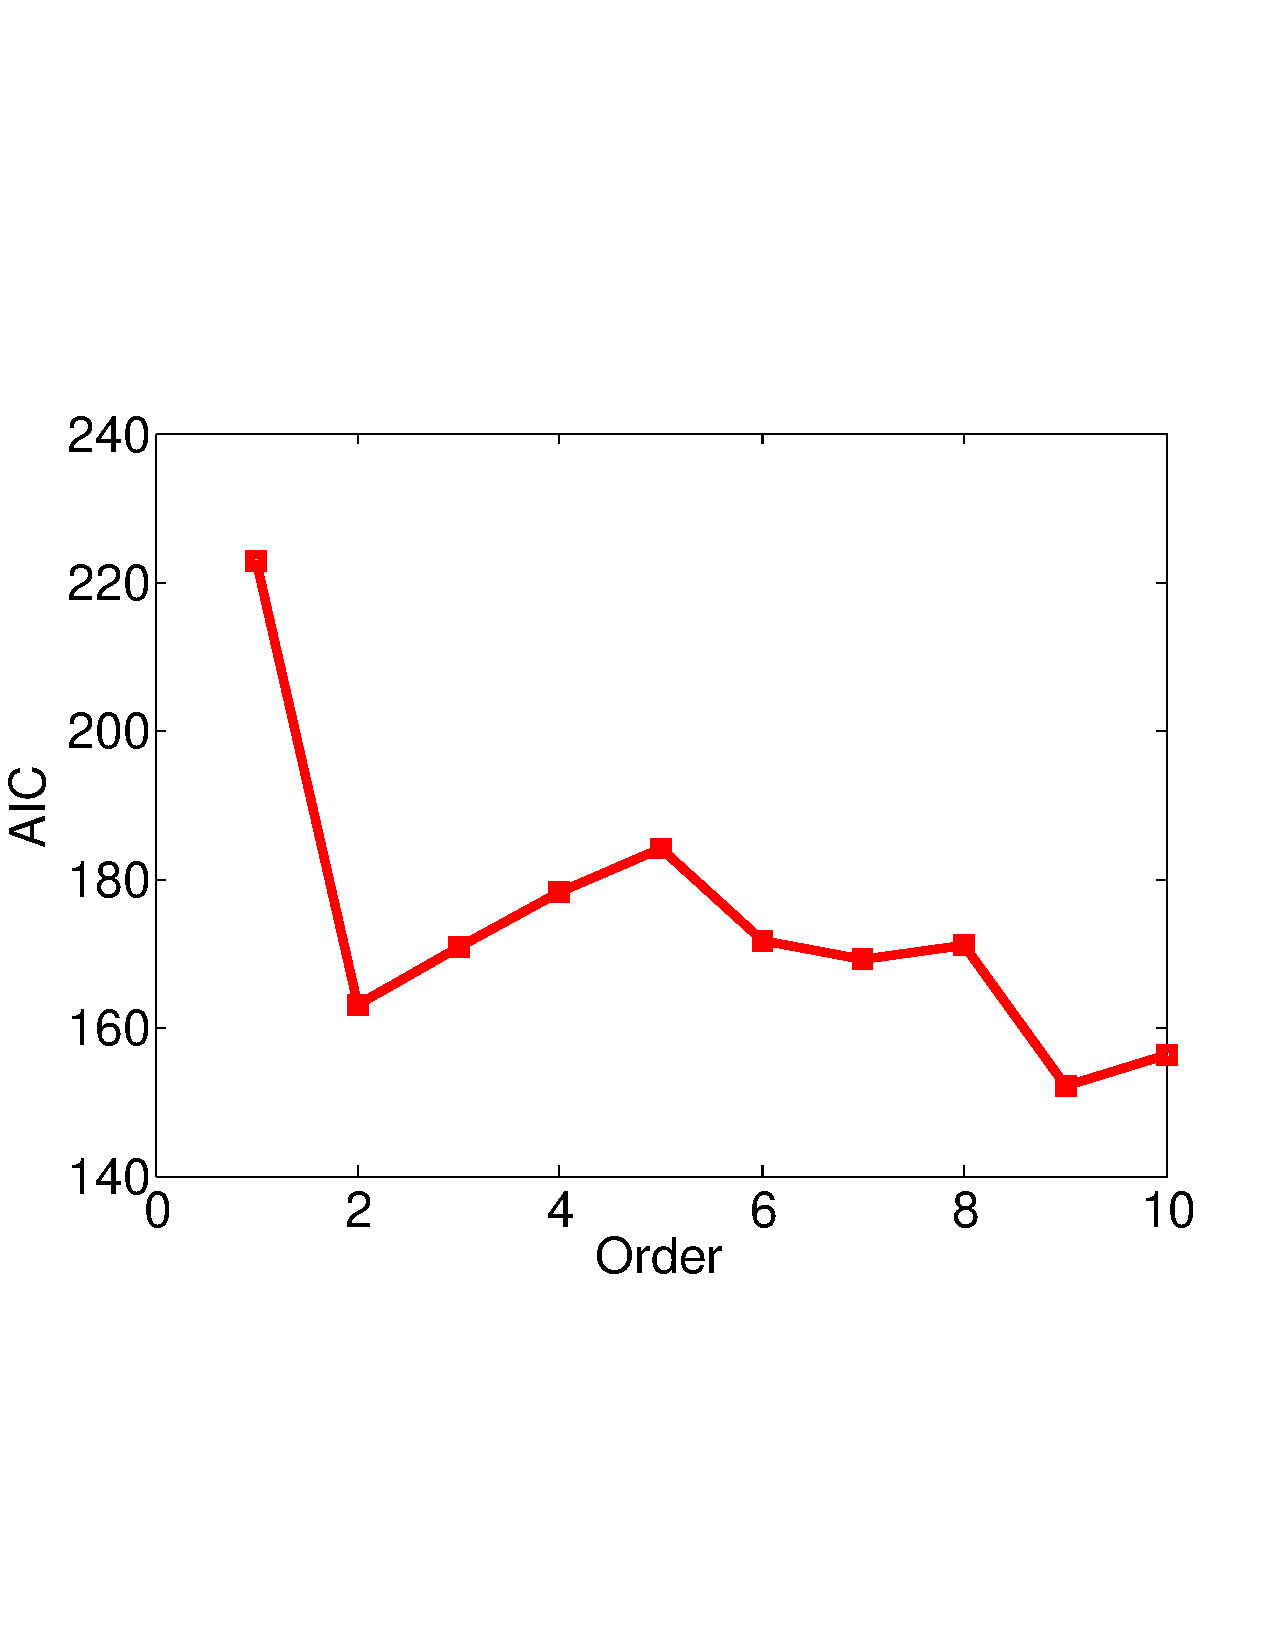
\includegraphics[width=3.0in]{AIC}
\vspace{-2cm}
\centering\caption{the relationship between AIC value and the chosen order.}
\label{figzh1}
\end{figure}


\paragraph*{Causality value}

   In the last part,we confirm the optimal order of the model of the lung cancer mortality and the aerosol extinction coefficient is 9.According to the best lag order and the definition of granger causality and new causality,we analyse the value of GC equals to 0.9346,the value of NC equals to 0.0515.As the both value of GC and NC are greater than 0,thus we say lung cancer mortality and AEC has a certain causal relationship.

\paragraph*{Significance test}
 In order to prove the causality value when order equals to 9 is of significance,we should take significance test for the two causality values.

 Significance test can be simply described as follows:when calculating the causality from $X_2$ to $X_1$,we should first randomly shuffle the $X_2$,then calculate the causality from $X_2$(shuffled sequence) to $X_1$.Repeat this process 100 times,then we get 100 GC values and NC values.Secondly,we separately rank the 100 GC values and 100 NC values from small to large. If the true value of GC or NC is larger than the 95th value of sorted GC value or NC value,then we say the Granger causality value or new causality value is of significance.

 Firstly,we randomly shuffle the $X_2$ which means the series of AEC,then calculate the causality value of $X_1$ and the shuffled $X_2$,repeat this process 100 times and rank the values from small to large.Results shown as follows:

\begin{figure}[htbp]
%\psfrag{iEEG}[c][c][2]{${\rm iEEG}$}
\vspace{-2.2cm}
\centering
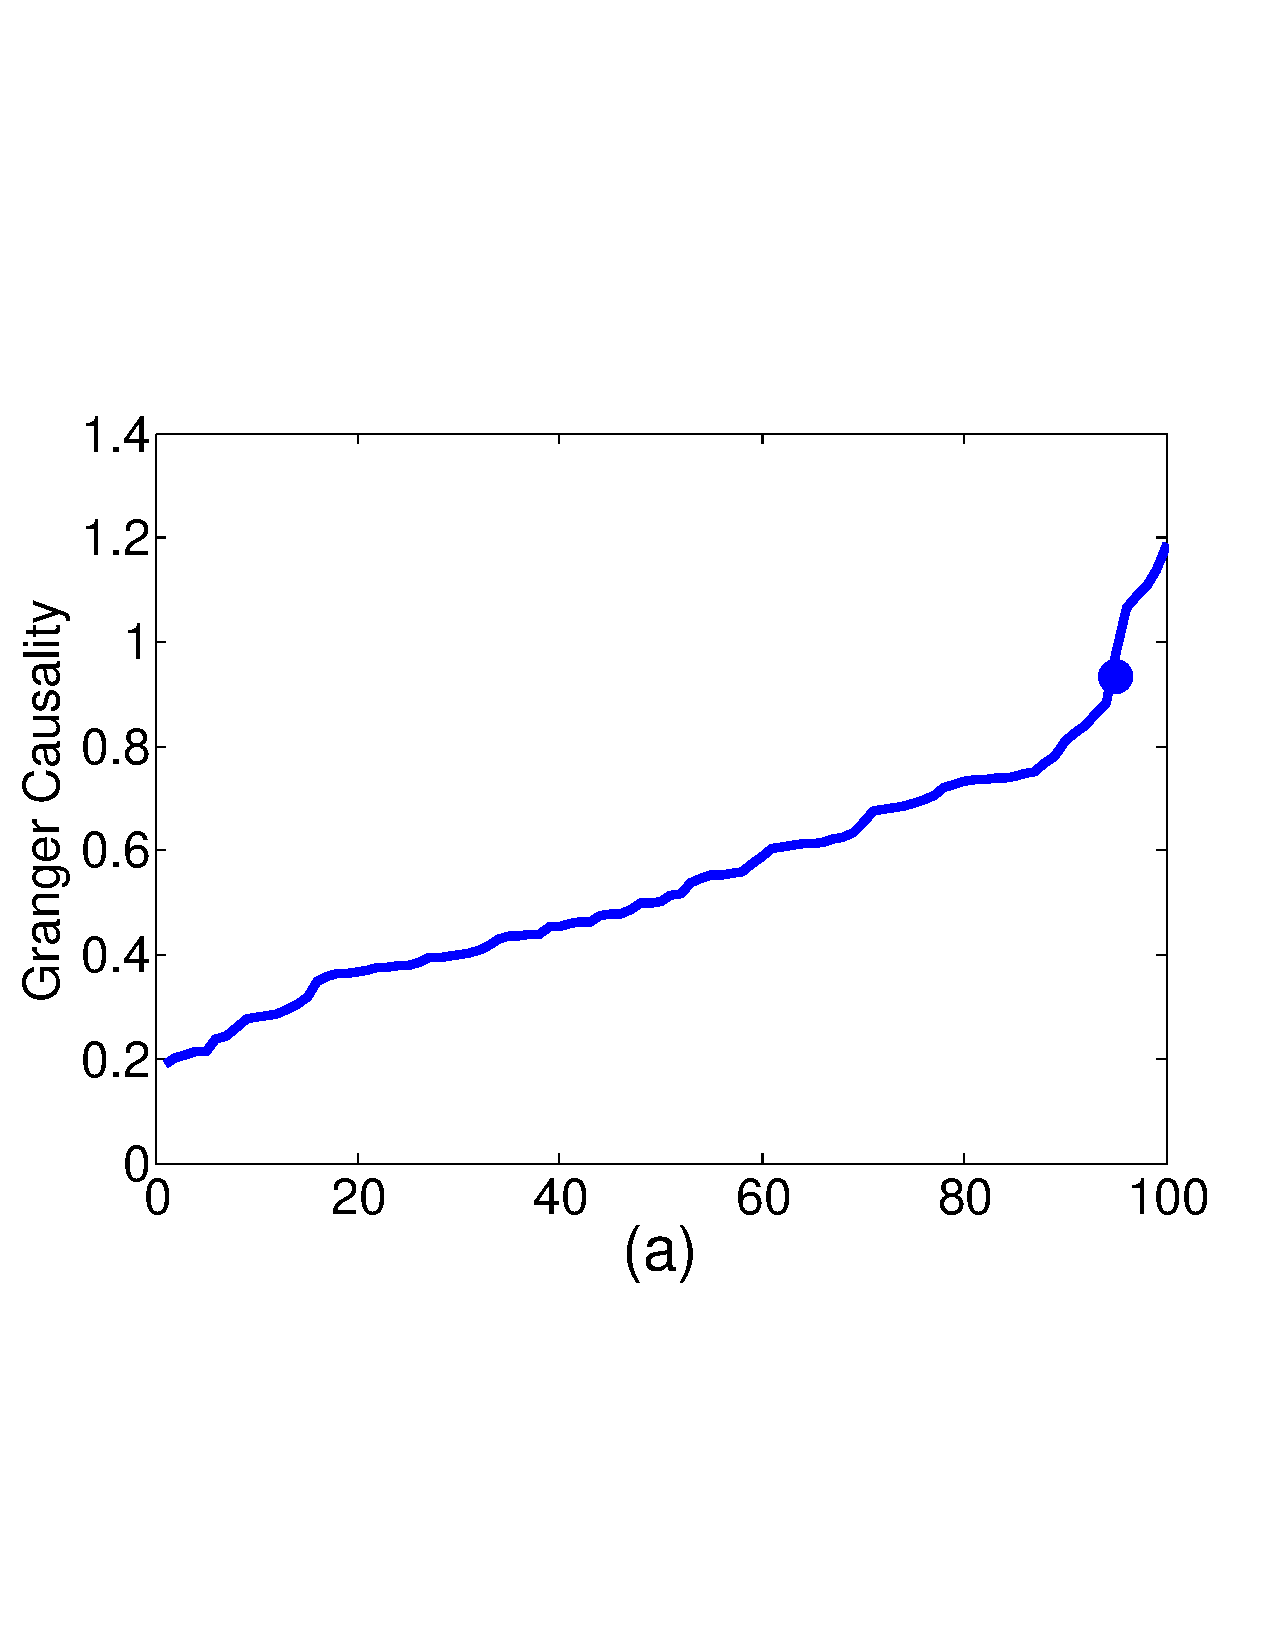
\includegraphics[width=3in]{significanceIndentifyGC2}\hspace{-0.2cm}
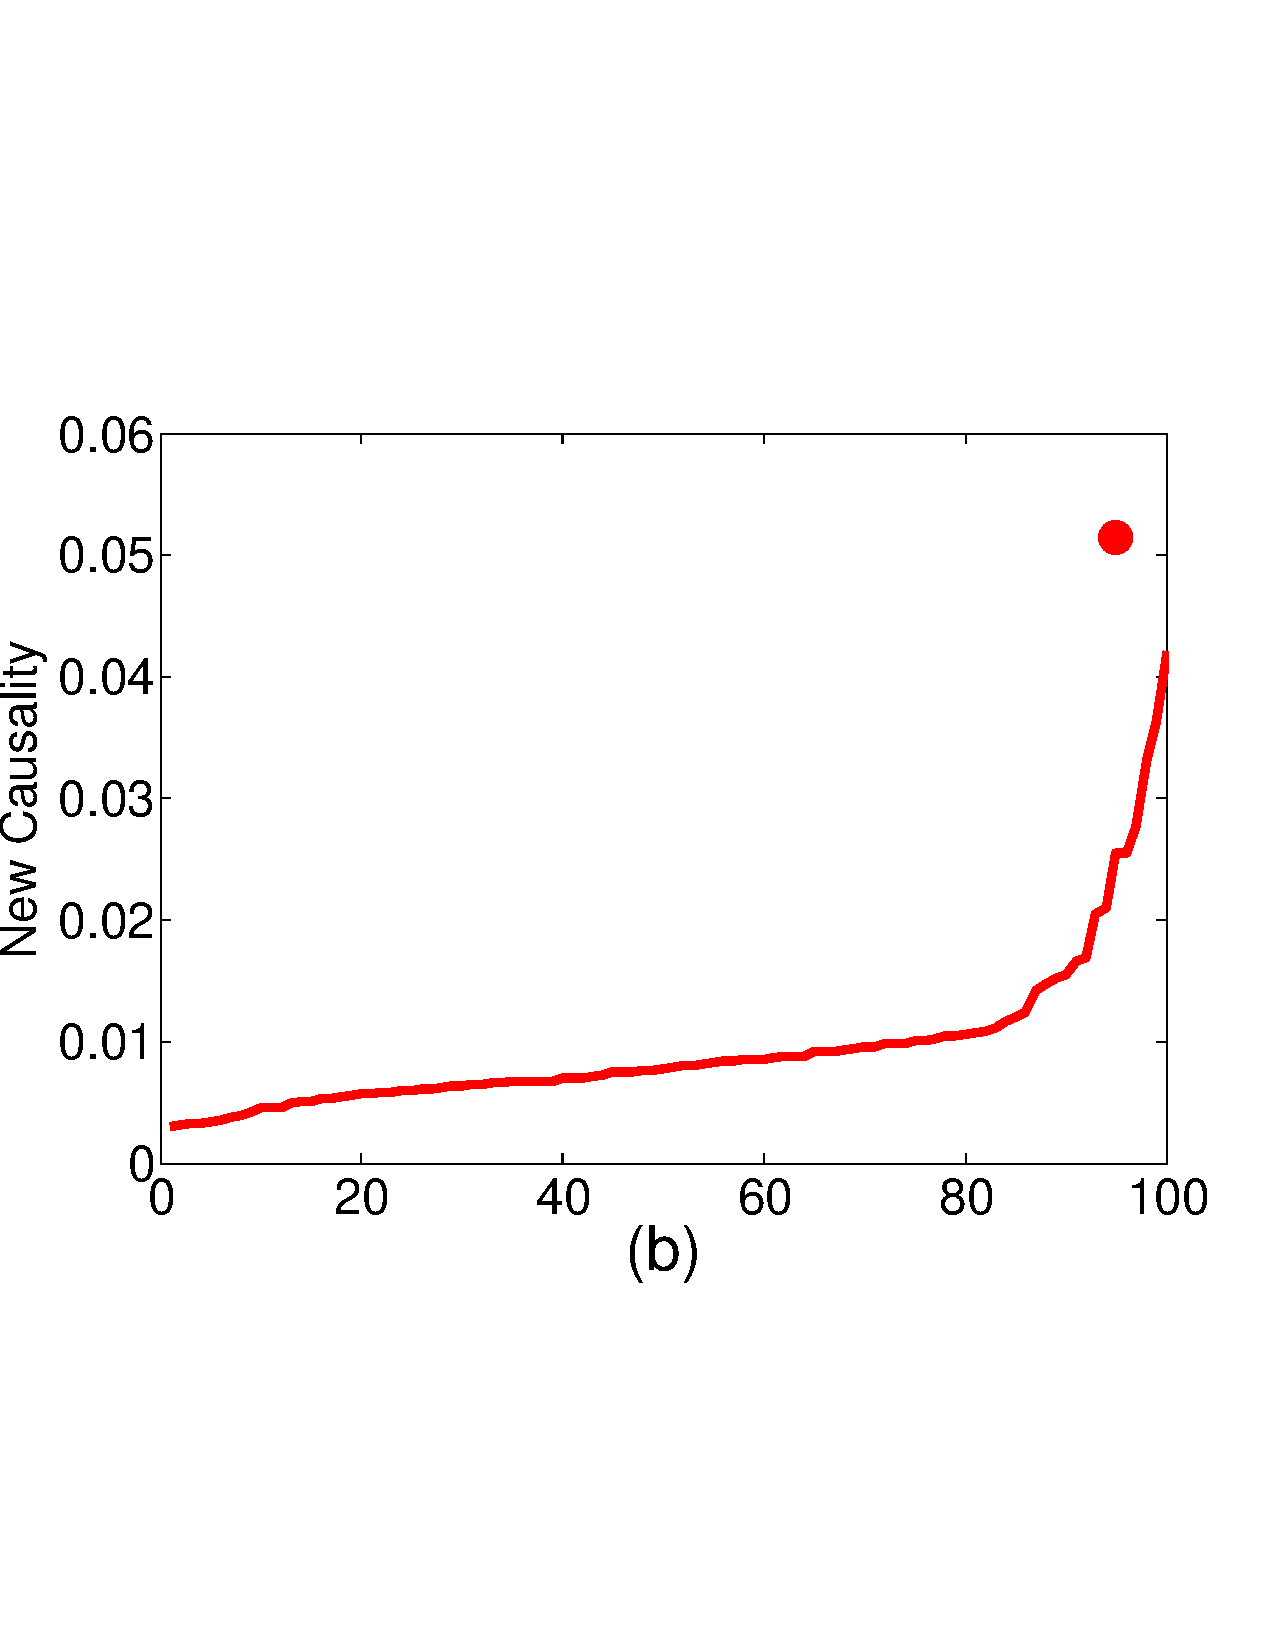
\includegraphics[width=3in]{significanceIndentifyNewCausality2}
\vspace{-2cm}\\
\caption{Significance Test for:(a) Granger Causality. (b) New Causality.}
\label{f6}
\end{figure}

We can see from the (Fig. 3),as we randomly shuffle the $X_2$ 100 times,we get 100 GC values and 100 NC values.After we rank this 100 NC and GC values from small to large,100\% of NC values is smaller than the true NC value(original $X_2$ series),94\%(less than 95\%) of GC values is smaller than the true GC value.Thus,causality value calculated by using Granger causality is not of significance.Conversely,NC value is of great significance.

\paragraph*{The confirm of the lag relationship between cause and effect.}
According to what we say above,the optimal order of the model is 9,we see from the formula (5) or (6),when order equals to 9,the numerator of new causality  $\sum\limits_{t=m+1}^{N}{(\sum\limits_{j=1}^{m}a_{12,j}X_{2,t-j})}^2$ contains 9 parts,in order to confirm the lag relationship between two time series,that is to confirm which part plays vital role to the NC value.The value of different lag year of j can be calculated by the formula(10),the results are shown as figure 4:

 \begin{equation}
 lagYear(j)=\sum_{t=10}^{40}(a_{12,j}X_{2,t-j})^2
\end{equation}

\begin{figure}[htbp]
%\psfrag{iEEG}[c][c][2]{${\rm iEEG}$}
\vspace{-2.2cm}
\centering
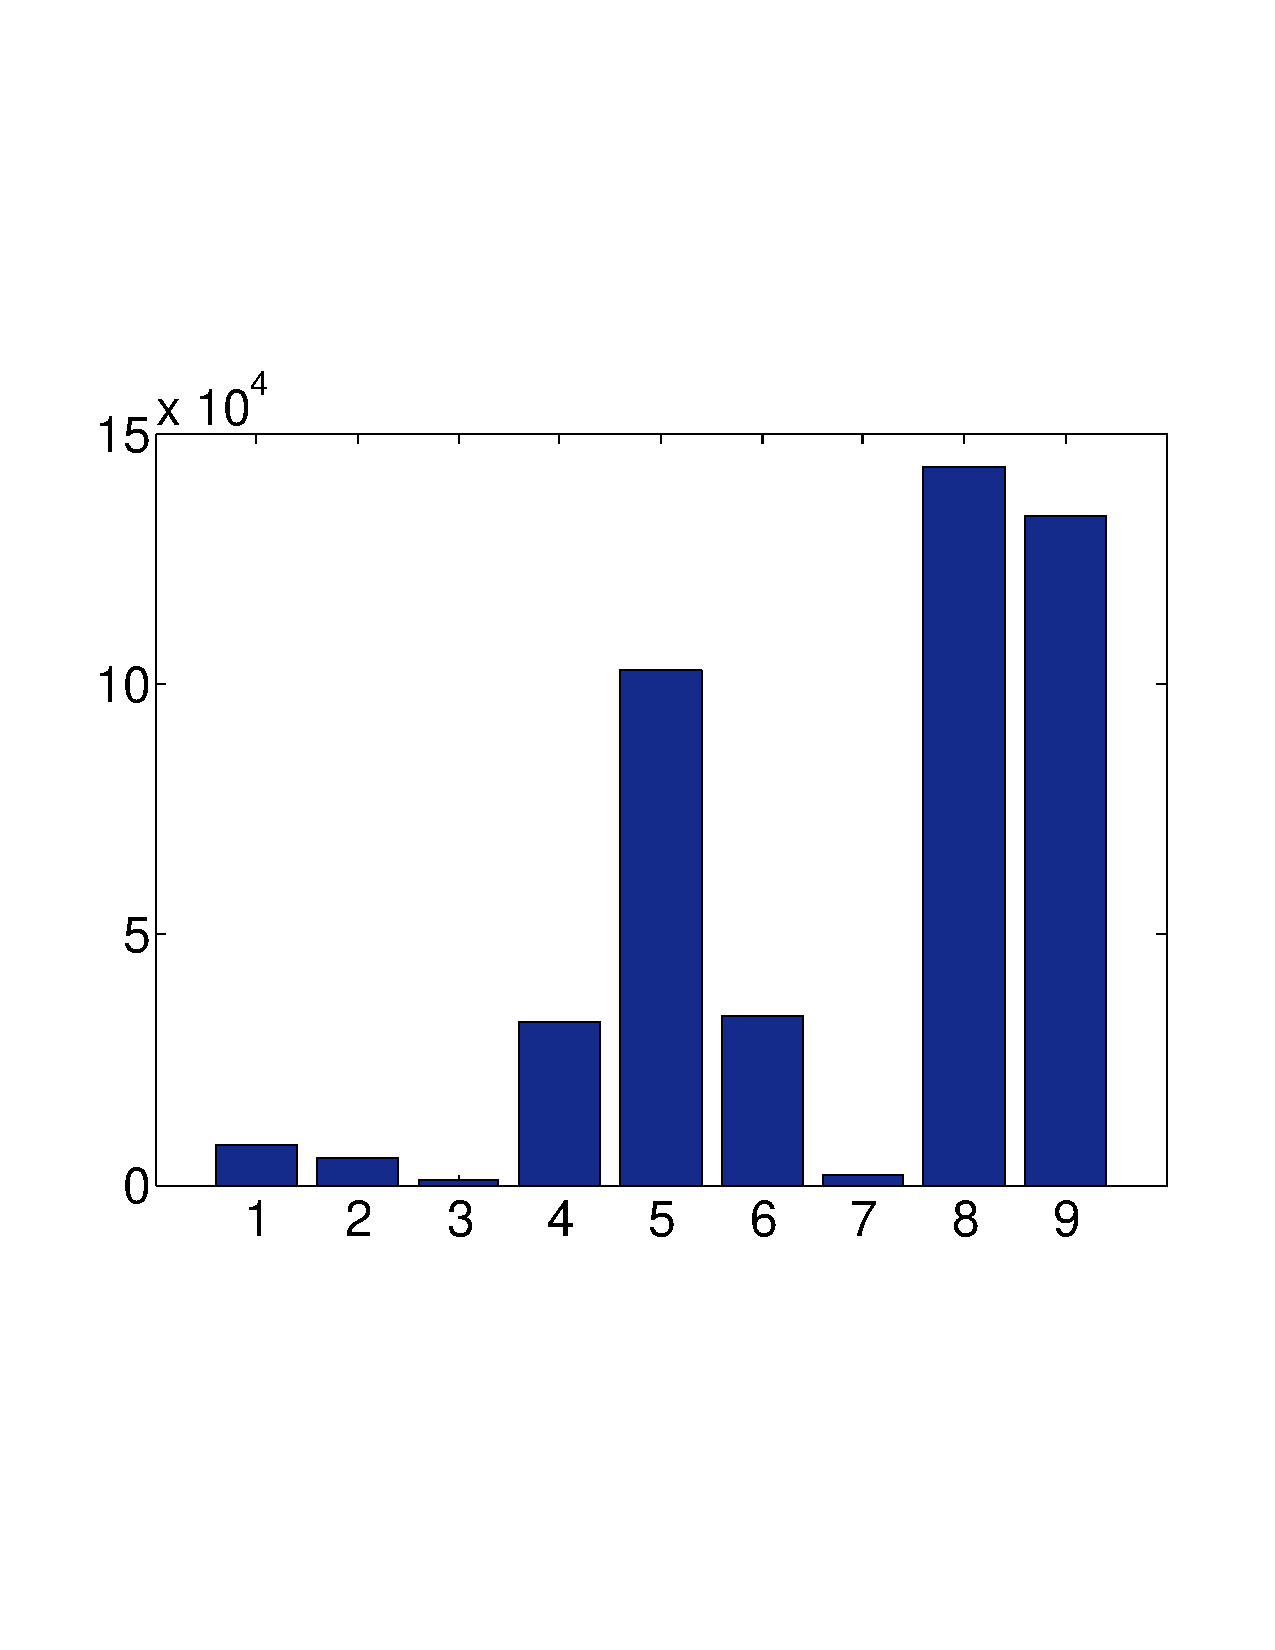
\includegraphics[width=3.0in]{ervryPart1_9}
\vspace{-2cm}
\centering\caption{The value of each part when order equals to 9.}
\label{figzh1}
\end{figure}

the count of lag j years part takes among the total lag year can be defined as:

 \begin{equation}
 countPart(j)=\frac{\sum\limits_{t=10}^{40}(a_{12,j}X_{2,t-j})^2 }
 {\sum\limits_{j=1}^{9}{(\sum\limits_{t=10}^{40}a_{12,j}X_{2,t-j})}^2}
\end{equation}

\begin{figure}[htbp]
%\psfrag{iEEG}[c][c][2]{${\rm iEEG}$}
\vspace{-2.2cm}
\centering
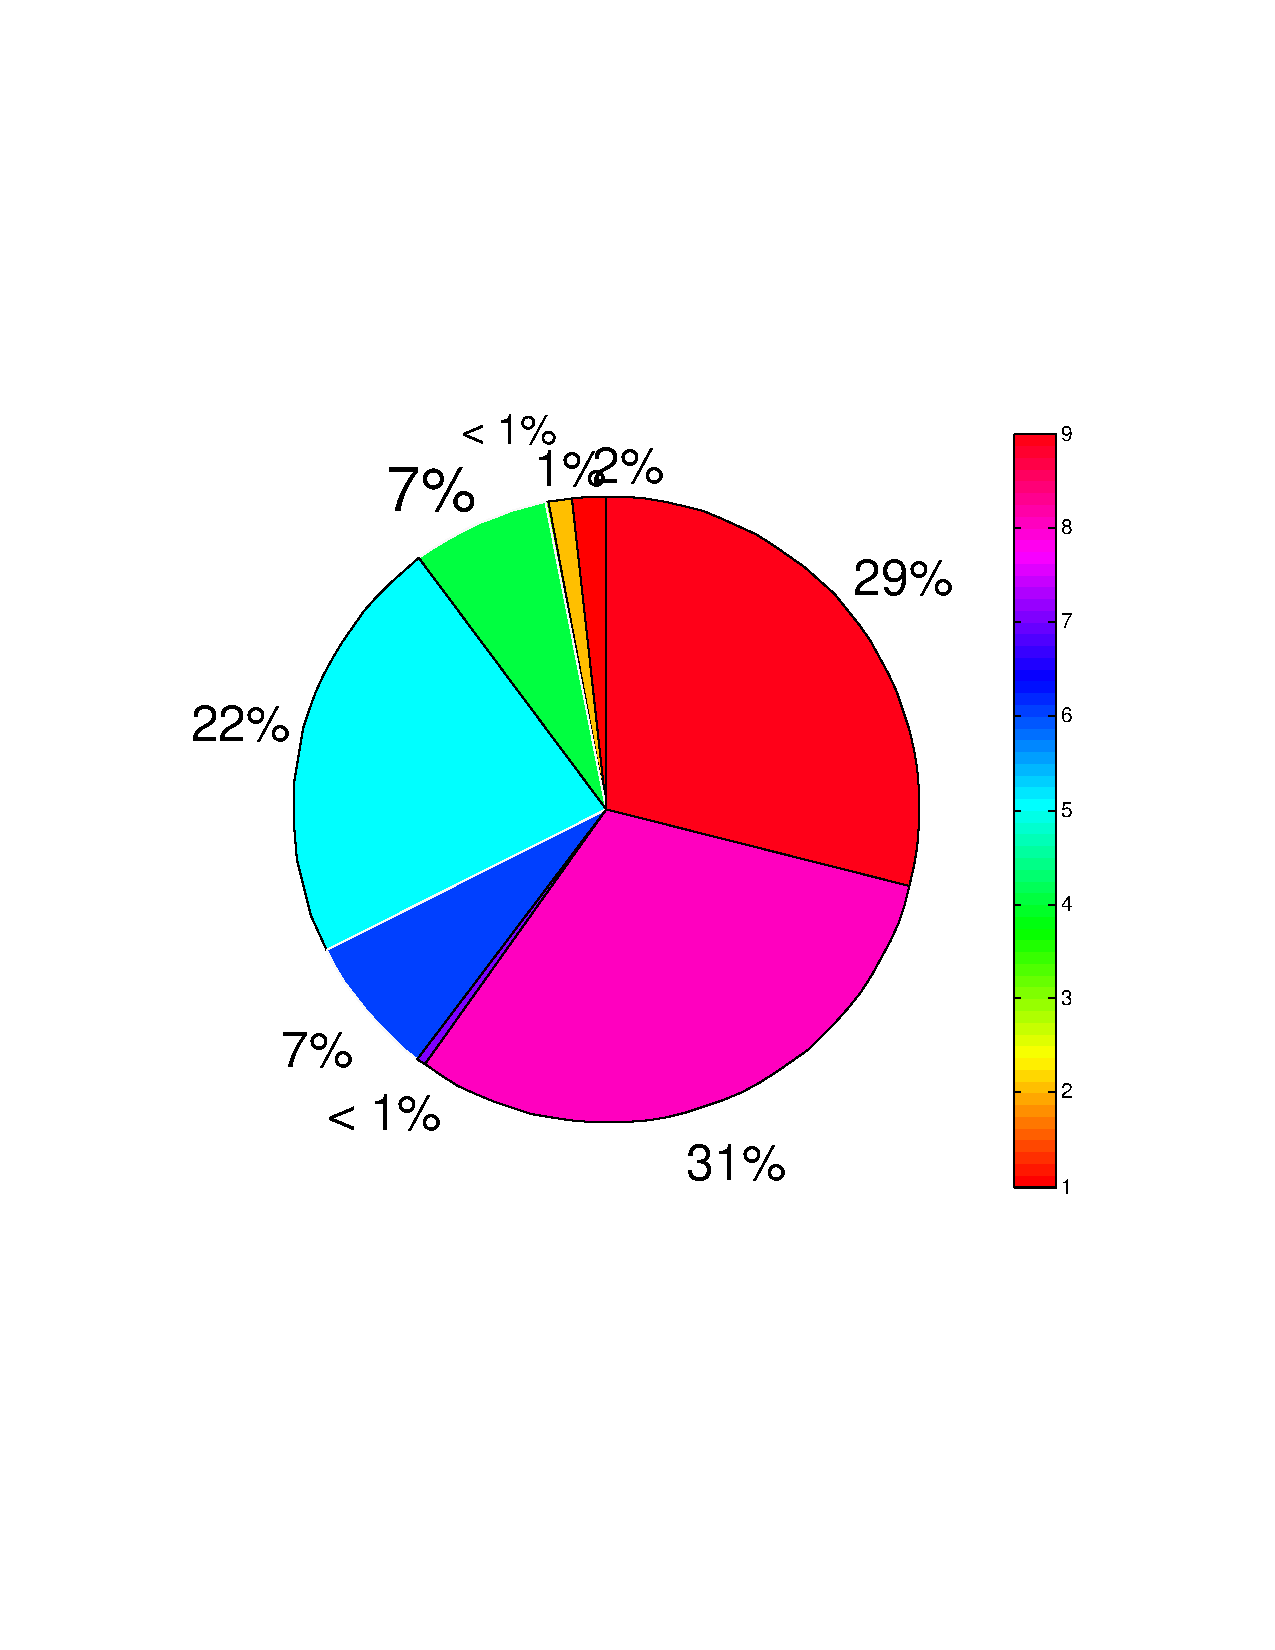
\includegraphics[width=3.0in]{pie}
\vspace{-2cm}
\centering\caption{when order equals to 9,the percentage of every part takes.}
\label{figzh1}
\end{figure}

As is shown in the (Fig. 5),when the order equals to 9,the eighth part takes most part,thus we can conclude the lung cancer mortality has eight years lag time relationship with aerosol extinction coefficient.That is to say,the rapid increasing trend of aerosol extinction coefficient will result in the high rate of lung cancer mortality after 8 years.

In order to prove AEC at low concentration leads to lung cancer with longer lag time, AEC at high concentration leads to lung cancer with shorter lag time,we divide the AEC 10-year running mean values into three parts,first part is from the year of 1960 to 1970(AEC is at low level),the year from 1971 to 1981 as the second part(AEC is at rapid rising trend),1982 to 1992 as the third part(AEC is at high level and is relatively stable).By comparing the causality value of AEC and the lung cancer mortality of different part to confirm the causal lag relationship between lung cancer and AEC.Here,we take the first part as example,the Granger causality value and new causality value when lag time equals to 0 (the data of AEC is from 1960-1970,the data of lung cancer mortality is from 1960-1970) can be analysed by using the formula (3) and (5),we define AEC as the $X_2$ sequence,lung cancer mortality as the $X_1$ sequence,when lag time equals to 1,the data of AEC starts from 1960 to 1970,the lung cancer mortality data begins at 1961 to 1971,at the same way,we can get one GC value and one NC value.By that analogy,similarly we can get different lag year's GC and NC value of the second part($X_1$ is from the year of 1971 to 2001,$X_2$ is from 1971 to 1981 and the length of $X_2$ is fixed.If the lag time equals to 0,we use the data of $X_1$ from 1971 to 1981.If the lag time equals to 1,we use the data of $X_1$ from 1972-1982,the rest can be done in the same manner,the last group of $X_1$ is from 1991 to 2001,the lag time between two series is 20 years).For the Last part,we first fix the length of $X_2$ from the year of 1982 to the year of 1992 which represents the high level of AEC,the first group of $X_1$ is from the year of 1982 to 1992,the results of two series indicate the GC and NC value of lag year equals to 0,the last group of $X_1$ is from 1991 to 2001,the lag time is 9 years.What we say above can be formulized as follows:($L$ indicates lung cancer mortality,$i$ should be integer)
 \begin{flushleft}
 $(1)Lag(i)=GC/NC(L(1960:1970),AEC((1960+i):(1970+i))) (-1<i<32)$
 \end{flushleft}

  \begin{flushleft}
 $(2)Lag(i)=GC/NC(L(1971:1981),AEC((1971+i):(1981+i))) (-1<i<22)$
   \end{flushleft}

\begin{flushleft}
 $(3)Lag(i)=GC/NC(L(1982:1992),AEC((1982+i):(1992+i))) (-1<i<10)$
   \end{flushleft}
 The results are shown below:

\begin{figure}[htbp]
%\psfrag{iEEG}[c][c][2]{${\rm iEEG}$}
\vspace{-2.2cm}
\centering
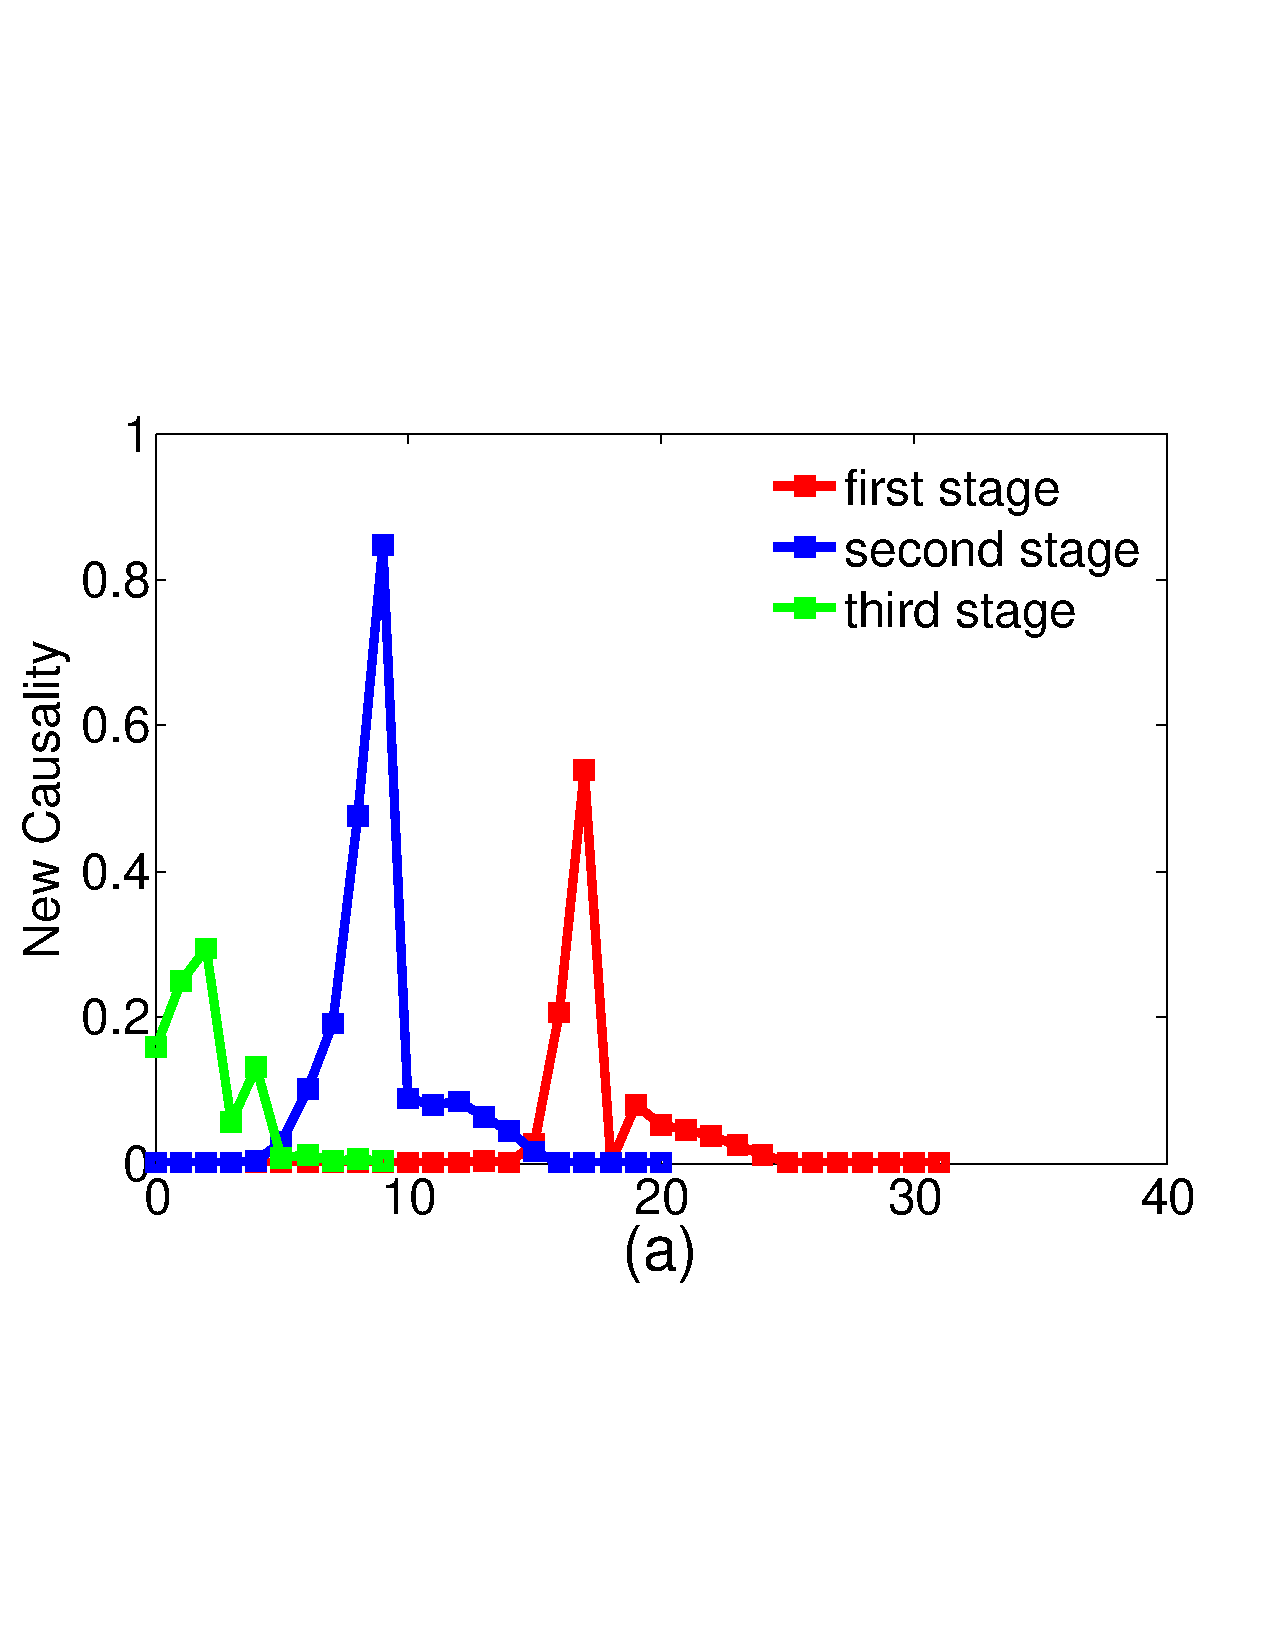
\includegraphics[width=3in]{newCausalityFenDuan2}\hspace{-0.2cm}
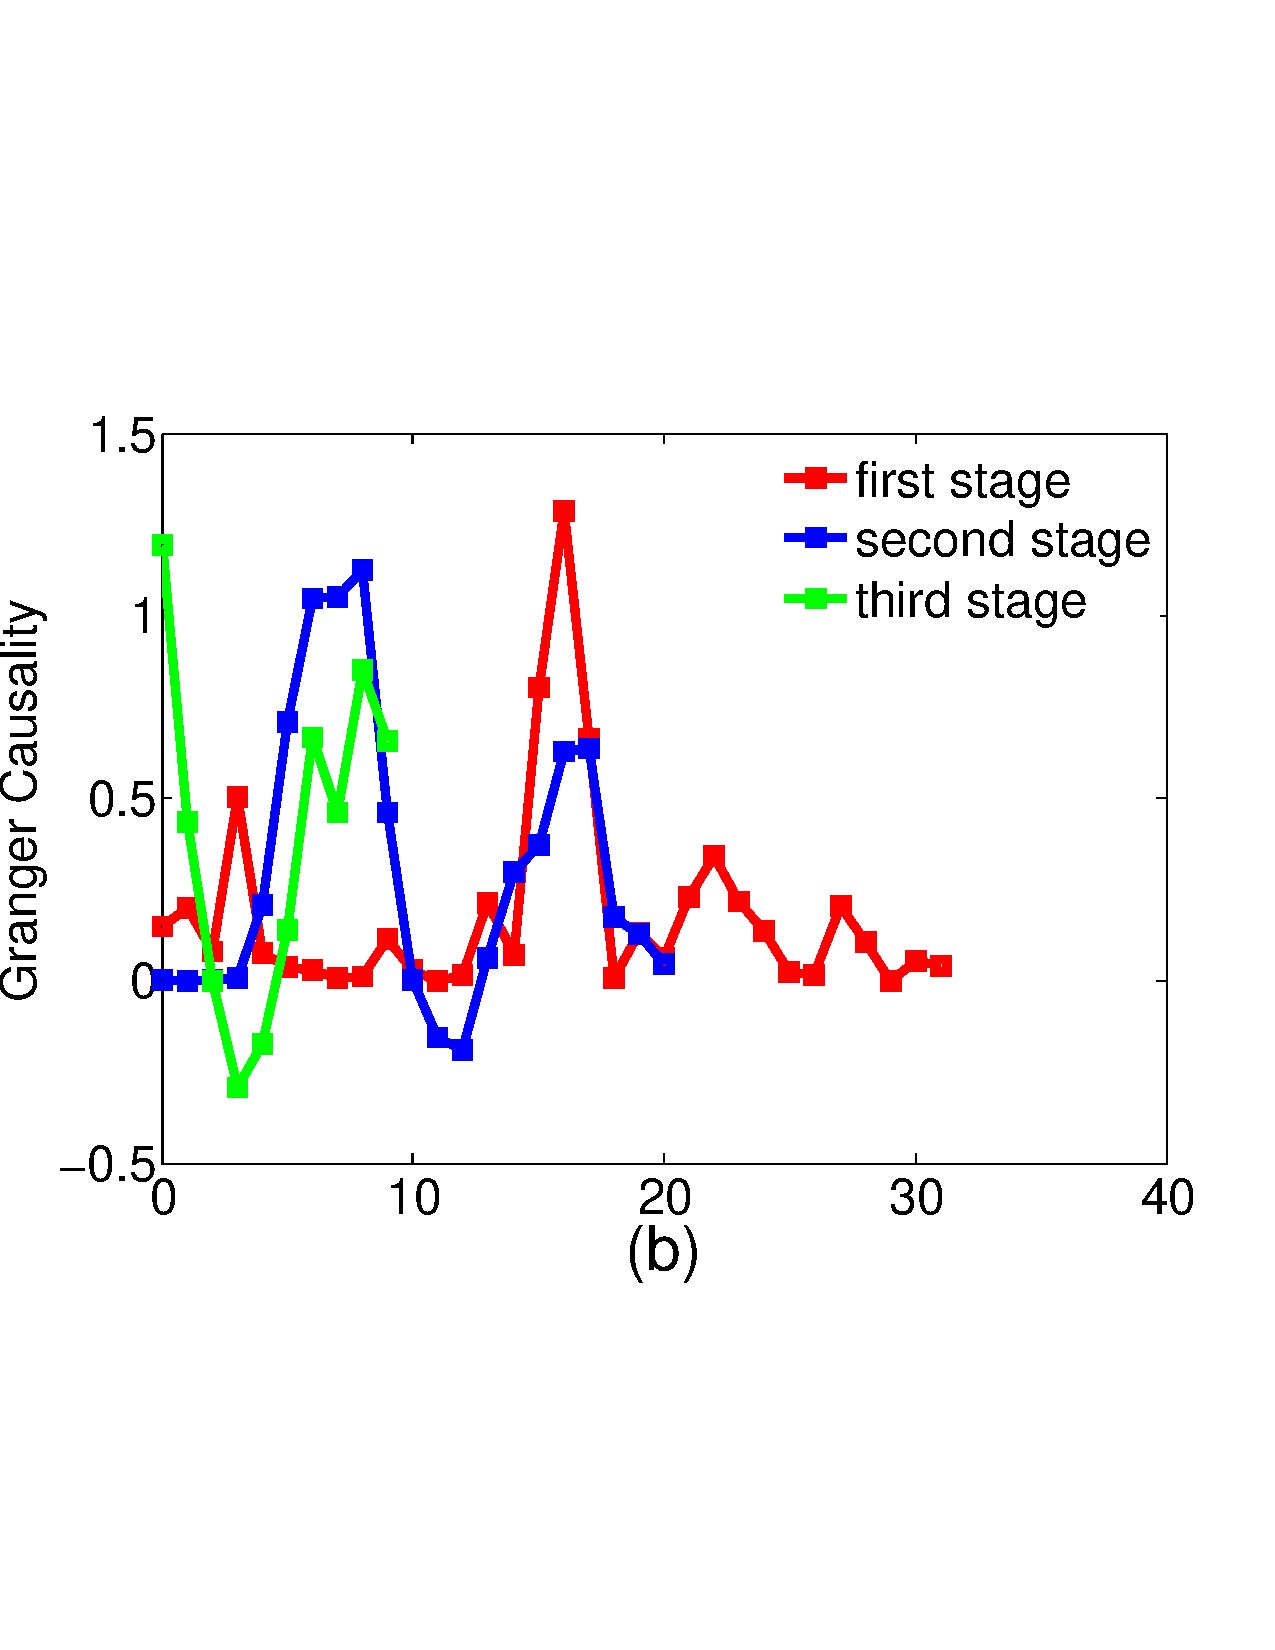
\includegraphics[width=3in]{grangerCuFenDuan}
\vspace{-2cm}\\
\caption{Lung cancer mortality and AEC's: (a) New Causality value. (b) Granger Causality value. }
\label{f6}
\end{figure}


We can see from the (Fig. 6),the red line represents the first stage where the AEC is at low level,the blue line indicates the second stage where AEC is at rising trend and the green line shows the tendency of high level of AEC.We see as the concentration of AEC enhances,the lag time decreases(the peak value appears earlier:(a)on the first stage,the maximum value of NC is when the lag time equals to 17 years;on the second stage,the maximum value of NC appears in the lag year equals to 9;on the third stage,the maximum value of NC is when the lag year time equals to 2.(b)The value of the first phase of the GC presents biggest in the lag time of 16 years,the maximum value of GC in second stage appears in the lag time of 8 years,the maximum value of GC in third stage appears in the lag time of 0 year.).

\paragraph*{Lag correlation.}
  In this subsection, we will analysis the correlation between lung cancer mortality and AEC.Correlation is one of the most common ways to analyse the relationship between two quantitative variables which quantifies the strength of the linear relationship.Correlation is not equal to causality, but it reflects the correlation direction and correlation degree between two variables. So it is very meaningful to our conclusion.Lag correlation shows the correlation between two variables when they lag different time.By analysing historical surface measurements of aerosol extinction coefficient in the Chinese city of Guangzhou,and show that the dramatic increase in the occurrence of air pollution events has been followed by a large enhancement in the incidence of lung cancer. By using the theory of correlation,Dui Wu and his team conclude that lung cancer
incidence and aerosol extinction coefficient are better correlated when a time lag of 7-8 is adopted which raise a heated discussion among Chinese.
  Here we use the conception of correlation,similarly,we use the same division means to analyse the coefficient of different lag year.($L$ indicates lung cancer mortality,$i$ should be integer)

    \begin{flushleft}
 $(1)Lag(i)=corrcoef(L(1960:1970),AEC((1960+i):(1970+i))) (-1<i<32)$
 \end{flushleft}

  \begin{flushleft}
 $(2)Lag(i)=corrcoef(L(1971:1981),AEC((1971+i):(1981+i))) (-1<i<22)$
   \end{flushleft}

\begin{flushleft}
 $(3)Lag(i)=corrcoef(L(1982:1992),AEC((1982+i):(1992+i))) (-1<i<10)$
   \end{flushleft}


\begin{figure}[htbp]
%\psfrag{iEEG}[c][c][2]{${\rm iEEG}$}
\vspace{-2.2cm}
\centering
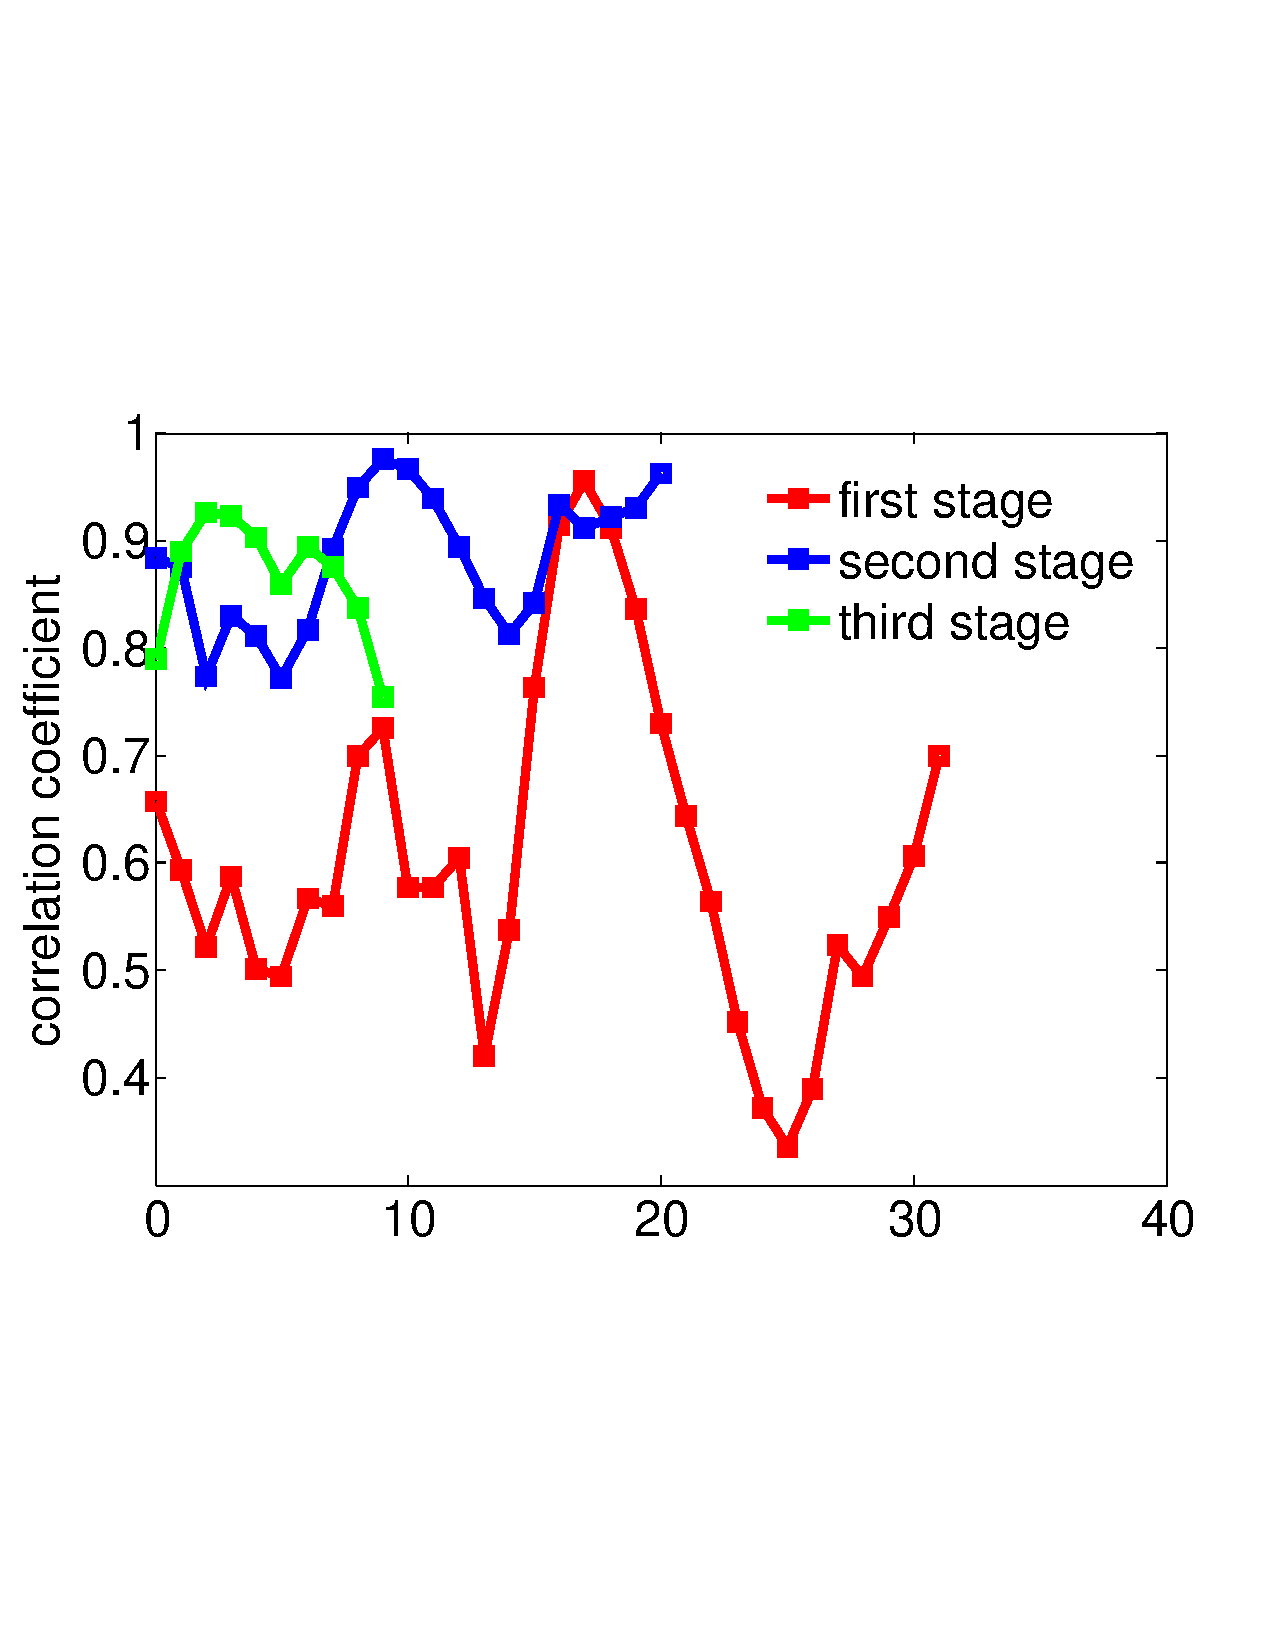
\includegraphics[width=3.0in]{corrcoeff}
\vspace{-2cm}
\centering\caption{The correlation coefficient of lung cancer mortality and AEC}
\label{figzh1}
\end{figure}

We can see from the (Fig. 7),the value of the first phase of the correlation coefficient presents biggest in the lag time of 16 years,the maximum value of correlation coefficient in second stage appears in the lag time of 9 years,the maximum value of correlation coefficient in third stage appears in the lag time of 2 years.The results are same as NC method.At the same time we see in the third stage,that is in the high concentration AEC level,the peak of the GC value appears in the lag time of 0 years which doesn't correspond to reality,the peak of the NC value appears in the lag time of 2 years and is consistent with the correlation method.From this,we can say the NC method is more accurate to reveal true reality than GC method.Our finding provides more evidence to use new causality method instead of Granger causality method.


\section*{Conclusions}

As we are unable to obtain corresponding data of other provinces or cities,we only take Guangzhou city in China as example.We apply the new causality method to confirm the 8 years lag relationship between lung cancer and aerosol particles which is consistent with the conclusion made by Dui Wu.Also we confirm that AEC at low concentration leads to lung cancer with longer lag time,AEC at high concentration leads to lung cancer with shorter lag time.The conclusion is consistent with the correlation analysis.The Granger causality can not get such conclusion,thus adding new evidence that new causality is more accurate than Granger causality to reveal the causal relationship.In the face of growing number of  patients with lung cancer and the deteriorative environment,people can not help but ask is the grey haze a factor of the rapid trend of lung cancer(as the main component of grey haze is aerosol particles)?The conclusion of this paper effectively confirmed this fact.In recent decades,with China's rapid economic development,China has obtained the remarkable economic achievements.However,this rapid growth accompanied by serious break of the natural environment,our health is suffering from the threat of the deteriorating environment.The conclusion of this passage is undoubtedly to tell people the necessity and urgency to manage the deteriorating environment.Clean air is the most basic human survival demand,everyone is equal to breath air.Policy makers should be determined to take all possible measures to strengthen the governance of the grey haze environmental and strengthen the collaboration between the meteorological departments and environmental protection to set up and improve early warning mechanism of the grey haze weather,remind people don't go outside when the grey haze weather,at the same time,taking necessary precautions is rather important.Otherwise we will soon pay a heavy price for blood.

\section*{References and Notes}

\bibliography{scibib}

\bibliographystyle{Science}

% Following is a new environment, {scilastnote}, that's defined in the
% preamble and that allows authors to add a reference at the end of the
% list that's not signaled in the text; such references are used in
% *Science* for acknowledgments of funding, help, etc.

\begin{scilastnote}
\item[1.] X. Tie, D. Wu, G. Brasseir, {\it Atmospheric Environment\/} {\bf 43}, 2375 (2009).
\item[2.] S. Hu, G. Dai, G. Worrell, Q. Dai, and H. Liang, {\it IEEE Trans Neural Networks\/} {\bf 22}, 829 (2011).

\item[3.] C. W. J Granger, {\it Econometrica} {\bf 37}, 424 (1969).

\item[4.] M. Ding, Y. Chen, S. Bressler, {\it Design Automation, 2006. Asia and South Pacific Conference on IEEE}, pp. 826-831.

\item[5.] C. Iii, R. Burnett, M. Thun et al., {\it Jama the Journal of the American Medical Association} {\bf 287}, 1132(2011).

%LUNG cancer,cardiopulmonary mortality and long-term exposure to fire particulate air pollution
\item[6.] D. Abbey, N. Nishino, W. Mcdonnell, et al., {\it  American Journal of Respiratory \& Critical Care Medicine} {\bf 159}, 373 (1999).

%Long-Term Inhalable Particles and Other Air Pollutants
%Related to Mortality in Nonsmokers
\item[7.] C. Goss, S. Newsom, J. Schildcrout, {\it American Journal of Respiratory \& Critical Care Medicine} {\bf 169}, 816 (2004).

%Effect of Ambient Air Pollution on Pulmonary
%Exacerbations and Lung Function in Cystic Fibrosis
\item[8.] O. Nielsen, Z. Andersen, R. Beelen et al., {\it Lancet Oncology} {\bf 14}, 813 (2013).
%Air pollution and lung cancer incidence in 17 European
%cohorts: prospective analyses from the European Study of
%Cohorts for Air Pollution Effects (ESCAPE)

\item[9.] F. Laden, J. Schwartz, F. Speizer et al., {\it American Journal of Respiratory \& Critical Care Medicine} {\bf 173}, 667 (2006).

    %Laden F, Schwartz J, Speizer FE, Dockery DW. 2006. Reduction
%in fine particulate air pollution and mortality: extended
%follow-up of the Harvard Six Cities study. Am J Respir Crit
%Care Med 173:667�C672.

\item[10.] O. Nielsen, Z. Andersen, M. Hvidberg et al., {\it Diseases of the Colon \& Rectum} {\bf 29}, 458 (1986).


%Raaschounielsen O, Andersen Z J, Hvidberg M, et al. Lung cancer incidence and %long-term exposure to air pollution from traffic.[J]. Diseases of the Colon & %Rectum, 1986, 29(7):458-458.

\item[11.] J. Mumford, X. He, R. Chapman et al., {\it Science} {\bf 235}, 217 (1987).

    %Mumford J L, He X Z, Chapman R S, et al. Lung cancer and indoor air pollution %in Xuan Wei, China.[J]. Science, 1987, 235(4785):217-20.

\item[12.] L. Lave, E. Seskin, {\it Science}  169 (1970).

    %Lave L B, Seskin E P. Air Pollution and Human Health The quantitative effect, %with an estimate of the dollar benefit of pollution abatement, is considered[J]. %Science, 1970, 169.


\item[13.] M. Chen, C. Lee, C. Hsu, {\it Economic Modelling} {\bf 28}, 526 (2011).


\item[14.] T. Ge, J. Feng, F. Grabenhorst, {\it Neuroimage} {\bf 59}, 1846 (2012).

\item[15.] Q. Gao, X. Duan, and H. Chen, {\it Neuroimage} {\bf 54}, 1280 (2011).

\item[16.] J. Zhu, Y. Chen, A. Lenonardson et al., {\it Plos Computational Biology} {\bf 6}, 157 (2010).

%Zhu J, Chen Y, Leonardson A S, et al. Characterizing Dynamic Changes in the Human %Blood Transcriptional Network[J]. Plos Computational Biology, 2010, 6(2):157-161.

\item[17.] J. B, {\it Tellus Series A-dynamic Meteorology \& Oceanography} {\bf 59}, 1846 (2007).

%Elsner J B. Granger causality and Atlantic hurricanes[J]. Tellus Series A-dynamic %Meteorology & Oceanography, 2007, 59(4):476�C485.

\item[18.] E. Kodra, S. Chatterjee, A. Ganguly, {\it Theoretical \& Applied Climatology} {\bf 104}, 325 (2011).

%Kodra E, Chatterjee S, Ganguly A R. Exploring Granger causality between global %average observed time series of carbon dioxide and temperature[J]. Theoretical & %Applied Climatology, 2011, 104(3):325-335.

\item[19.] S. Hu, H. Wang, J. Zhang, {\it IEEE Transactions on Neural Networks \& Learning Systems} (2015).

\item[20.] S. Hu, X. Jia, {\it IEEE Transactions on Neural Networks \& Learning Systems} (2015).

\item[21.] X. Tie, J. Cao, {\it Particuology} {\bf 7}, 426 (2009).

\item[22.] H. Akaike, {\it IEEE Transactions on Automatic Control} 716 (1974).


\item[23.] A. Seghouane, S. Amari, {\it IEEE Transactions on Neural Networks} {\bf 18}, 97 (2007).

\item[24.] H. Bozdogan, {\it Psychometrika} {\bf 52},345 (1987).


\end{scilastnote}


\section*{Acknowledgements}

This work was funded by National Natural Science Foundation of China under Grant No.61473110, National Science Foundation of Zhejiang Province, China, under Grant No. Z13F030002, International Science \& Technology Cooperation Program of China, Grant No.2014DFG12570, Key Lab of Complex Systems Modeling \& Simulation, Ministry of Education, China.



\end{document}




















